\section{Token, Length \& Char-Processing RNN}

Starting from the previous architecture, we developed this new \textsc{RNN}, represented in the image \ref{complex-rnn}, with the idea of feeding the network not only with the word\footnote{
    The same idea has been applied to the subwords as well.
} token but also with some other "metadata", namely:
\begin{itemize}
    \item the \textit{length} of the word (zero in case of punctuation symbols or markers)
    \item the \textit{char representation} of the word, i.e. a vector of fixed length, equal to the maximal length of a word from the \textit{Divine Comedy}, representing its char tokenization (or a vector of zeros in case of punctuation symbols or markers) which is then processed by a \textsc{GRU} layer\footnote{
        This obviously made it useless to try developing a \textit{Char-Level} variation for this architecture, as each char would have been processed separately. Thus, both due to this fact and some training problems encountered for the \textit{Char-Level} models, as well as their not-so-high scores obtained using the previous architecture, we decided not to develop them for future architectures anymore. 
    }
\end{itemize}

\begin{figure}[!hbt]
    \centering
    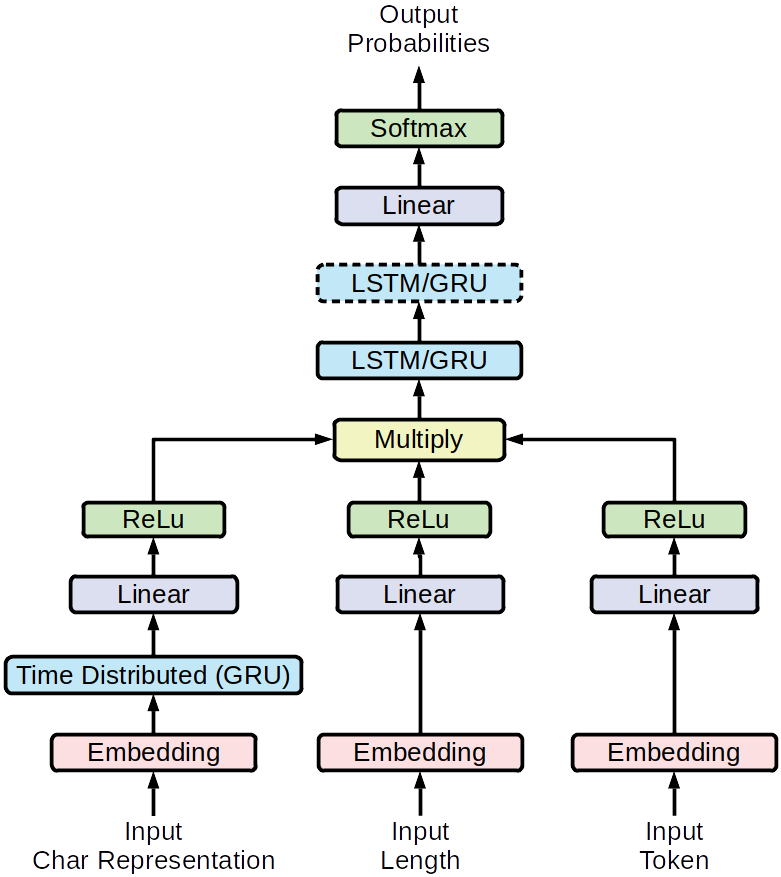
\includegraphics[scale=0.65]{images/model-2.png}%
    \caption{Token, Length \& Char-Processing RNN Architecture}%
    \label{complex-rnn}
\end{figure}

Thus, the final model is made of these three inputs, each of which is separately processed and whose results gets merged into a single vector of a given dimension, which is eventually fed to one or two recurrent layers and a final dense layer with softmax activation, exactly like the previous model.

\subsubsection{\textsc{Hyperparameters and Results}}

Again, here we had the same set of independent hyperparameters for both the variations of the models.
Still, differently from the previous architecture, this one had a larger number of them due to the higher number of inputs, namely:
\begin{itemize}
    \item The dimensions of the \textsc{Token Embedding} layer, the \textsc{Length Embedding} layer and the \textsc{Char Embedding} layer
    \item The dimension of the latent space prior to the \textsc{Multiply} layer 
    \item The kind of \textsc{RNN} (\textsc{GRU} or \textsc{LSTM})
    \item The number of \textsc{RNN} layers (either one or two), and their respective number of units
    \item The dropout rate of the \textsc{RNN} layers
\end{itemize}

After all the tests, this architecture showed scores similar to those of the previous architecture related to the \textit{Subword-Level} variation.
Instead, a slight increase could be noticed on the scores related to the \textit{Word-Level} variation, which were still a little worse than those of the \textit{Subword-Level}.

Given all of this, we decided not to investigate these basic models anymore and try some more recent kinds of architecture.